\subsection{Stability on non-smooth objectives}
\label{sec:stability}

\begin{figure}
%	%\begin{minipage}{0.61\textwidth}
\centering
%% \vspace{-2.25em}
  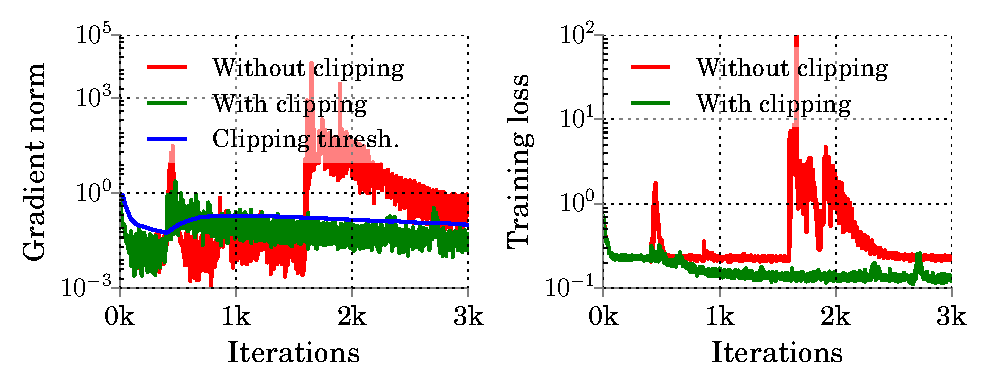
\includegraphics[width=\linewidth]{experiment_results/clipping_example.pdf} 
% \vspace{-0.75em}
\caption{A variation of the LSTM architecture in \citep{zhu2016trained} exhibits exploding gradients.
The proposed adaptive gradient clipping threshold (blue) stabilizes the training loss.}
\label{fig:stability}
%\end{minipage}
\end{figure}

The process of training neural networks is inherently non-stationary, with the landscape abruptly switching from flat to steep areas. 
In particular, the objective functions of RNNs with hidden units can exhibit occasional but very steep slopes \citep{pascanu2013difficulty,szegedy2013intriguing}.
To deal with this issue, gradient clipping has been established in literature as a standard tool to stabilize the training using such objectives \citep{pascanu2013difficulty,Goodfellow-et-al-2016,gehring2017convolutional}. 
%When that happens, the smoothed statistics from our measurement functions might not be representative.
%So, it is not always safe to assume that the smoothed statistics from our measurement functions so far will accurately represent the objective with abruptly large gradient in the next step.

We use \emph{adaptive gradient clipping} heuristics as a very natural addition to our basic tuner. 
However, the classic tradeoff between adaptivity and stability applies: 
setting a clipping threshold that is too low can hurt performance;
setting it to be high, can compromise stability.
\tuner, keeps running estimates of extremal gradient magnitude squares, $h_{max}$ and $h_{min}$ in order to estimate a generalized condition number.
We posit that $\sqrt{h_{max}}$ is an ideal gradient norm threshold for adaptive clipping.
In order to ensure robustness to extreme gradient spikes, like the ones in Figure~\ref{fig:stability}, we also limit the growth rate of the envelope $h_{max}$ in Algorithm~\ref{alg:curv_func} as follows:
\begin{equation}
 h_{max} 
 \leftarrow
 \beta \cdot h_{max}
 	+ (1-\beta) \cdot \textrm{min}\left\{
 		h_{max,t}, 100 \cdot h_{max}
 	\right\}
\end{equation}
Our heuristics follows along the lines of classic recipes like~\cite{pascanu2013difficulty}. However, instead of using the average gradient norm to clip, it uses a running estimate of the maximum norm $h_{\max}$. In Figure~\ref{fig:stability}, we demonstrate the mechanism of our heuristic by presenting an example of an LSTM that exhibits the 'exploding gradient' issue. The proposed adaptive clipping can stabilize the training process using \tuner and prevent large catastrophic loss spikes.  
\label{sec:infl_clip}
\begin{figure}
\centering
\begin{tabular}{c@{\hspace{0.0em}} c}
	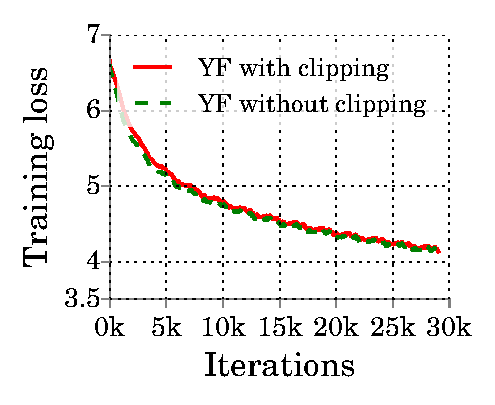
\includegraphics[width=0.49\linewidth]{experiment_results/ptb/clip_cmp.pdf} &
	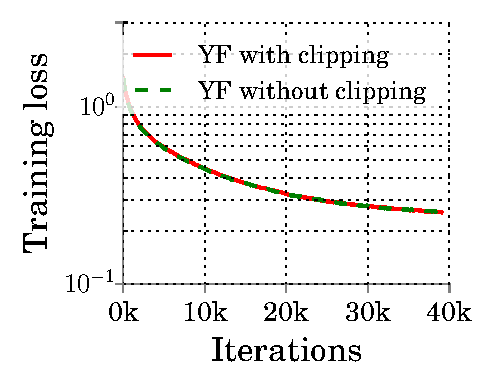
\includegraphics[width=0.49\linewidth]{experiment_results/resnet/cifar10_clip_cmp.pdf}
\end{tabular}
\caption{Training losses on PTB LSTM (left) and CIFAR10 ResNet (right) for YellowFin with and without adaptive clipping.}
\label{fig:infl_clip}
\end{figure}


%\begin{table*}
%\begin{minipage}{0.61\textwidth}
%\centering
%% \vspace{-2.25em}
%  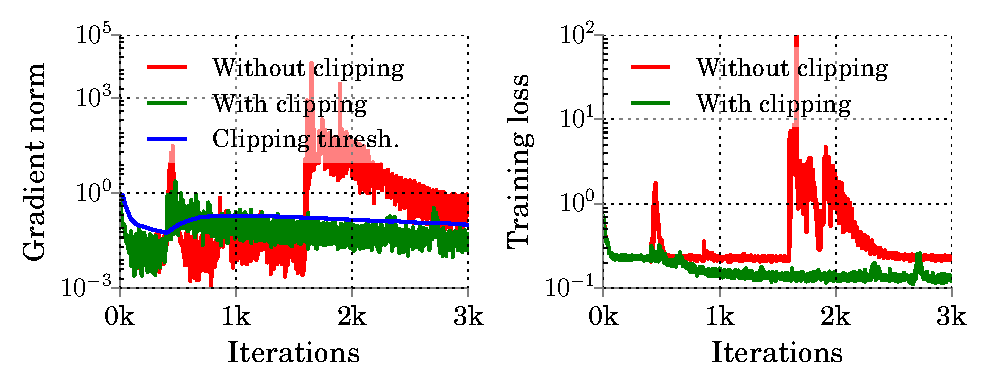
\includegraphics[width=0.95\linewidth]{experiment_results/clipping_example.pdf} 
% \vspace{-0.75em}
%\captionof{figure}{A variation of the LSTM architecture in \citep{zhu2016trained} exhibits exploding gradients.
%The proposed adaptive gradient clipping threshold (blue) stabilizes the training loss.}
%\label{fig:stability}
%\end{minipage}
%\begin{minipage}{0.01\textwidth}
%	 \ 
%\end{minipage}
%\begin{minipage}{0.37\textwidth}
%\centering
%%\small
%\vspace{0.5em}
%\begin{tabular} {@{\hspace{0.2em}}c | c | c @{\hspace{0.2em}}}
%\toprule
%	& Loss & BLEU4 \\
%\midrule
%\midrule
%	Default w/o clip. & \multicolumn{2}{c}{diverge} \\ [0.3em]
%	Default w/ clip. & 2.86 & 30.75 \\ [0.3em]
%	YF & \textbf{2.75} & \textbf{31.59} \\
%\bottomrule
%\end{tabular}
%\vspace{2.25em}
%\captionof{table}{German-English translation validation performance using convolutional seq-to-seq learning.}
%\label{tab:conv_seq}
%\end{minipage}
%%\vspace{-0.75em}
%\end{table*}

%Section~\ref{sec:oracles} describes the core measurement functions for \tuner tuner. To support its tuning rule, \tuner calculates smoothed, rough approximations of curvature ranges, a distance from a local minimum and gradient variance.
%Neural network objectives can involve arbitrary non-linearities, and large Lipschitz constants \citep{szegedy2013intriguing}.
%Furthermore, the process of training them is inherently non-stationary, with the landscape abruptly switching from flat to steep areas. 
%The process of training neural networks is inherently non-stationary, with the landscape abruptly switching from flat to steep areas. 
%In particular, the objective functions of RNNs with hidden units can exhibit occasional but very steep slopes \citep{pascanu2013difficulty,szegedy2013intriguing}.
%%When that happens, the smoothed statistics from our measurement functions might not be representative.
%%So, it is not always safe to assume that the smoothed statistics from our measurement functions so far will accurately represent the objective with abruptly large gradient in the next step.
%To deal with this issue, we use \emph{adaptive gradient clipping} heuristics as a very natural addition to our basic tuner. It is discussed with extensive details in Appendix~\ref{sec:adapt_clip}.  
%In Figure~\ref{fig:stability} in Appendix~\ref{sec:adapt_clip}, we present an example of an LSTM that exhibits the 'exploding gradient' issue. The proposed adaptive clipping can stabilize the training process using \tuner and prevent large catastrophic loss spikes.
%\begin{table}
%\centering
%\begin{tabular} { c | c | c | c}
%\toprule
%	& Default w/o clip. & Default w/ clip. & YF \\
%\midrule
%\midrule
%	Validation loss & diverge & 2.86 & 2.75 \\
%	Validation BLEU4 & diverge & 30.75 & 31.59 \\ 
%\bottomrule
%\end{tabular}
%\caption{German-English translation performance using convolutional sequence to sequence learning.}
%\label{tab:conv_seq}
%\end{table}

\begin{wrapfigure}[10]{r}{0.48\linewidth}
%asdfad
\hspace{-0.75em}
\begin{minipage}{\linewidth}
%%\begin{table}[h]
%\centering
\small
%\hspace{-1em}
\vspace{-0.75em}
\begin{tabular} {@{\hspace{0.1em}}c@{\hspace{0.3em}} | @{\hspace{0.35em}}c@{\hspace{0.4em}}c @{\hspace{0.1em}}}
\toprule
	& Loss & BLEU4 \\
\midrule
\midrule
	Default w/o clip. & \multicolumn{2}{c}{diverge} \\ [0.3em]
	Default w/ clip. & 2.86 & 30.75 \\ [0.3em]
	YF & \textbf{2.75} & \textbf{31.59} \\
\bottomrule
\end{tabular}
%\hspace{-1em}
\captionof{table}{German-English translation validation metrics using convolutional seq-to-seq model.}
%\vspace{2.25em}
\label{tab:conv_seq}
\end{minipage}
\end{wrapfigure}
We validate the proposed adaptive clipping on the convolutional sequence to sequence learning model \citep{gehring2017convolutional} for IWSLT 2014 German-English translation. The default optimizer~\citep{gehring2017convolutional} uses learning rate $0.25$ and Nesterov's momentum $0.99$, diverging to loss overflow due to 'exploding gradient'. It requires, as in~\citet{gehring2017convolutional}, strict manually set gradient norm threshold $0.1$ to stabilize. 
%We train the model for 120 epochs and report the best validation loss, as well as the best validation BLEU4 score. 
%We follow the default optimizer setting in~\citep{gehring2017convolutional}, where manually set strict clipping is applied before performing SGD with learning rate $0.25$ and Nesterov's momentum set to $0.99$. 
%The optimizer diverges when the clipping is removed. 
In Table~\ref{tab:conv_seq}, we can see YellowFin, with adaptive clipping, outperforms the default optimizer using manually set clipping, with 0.84 higher validation BLEU4 after 120 epochs. 
To further demonstrate the practical applicability of our gradient clipping heuristics, in Figure~\ref{fig:infl_clip}, we demonstrate that the adaptive clipping does not hurt performance on models that do not exhibit instabilities without clipping. Specifically, for both PTB LSTM and CIFAR10 ResNet, the difference between \tuner with and without adaptive clipping diminishes quickly. 
%Thinking fast and slow approach:
%- slow layer, the basic tuner we described
%- fast layer: applies clipping based on the statistics estimated
%- *and* we don’t let the estimates grow too quickly


%%%%%%%%%%%%%%%%%%% latest backup version %%%%%%%%%%%%%%%%%%%%%%%%%%%%%%%%%%%%%

%%\begin{table*}
%%\begin{minipage}{0.61\textwidth}
%%\centering
%%% \vspace{-2.25em}
%%  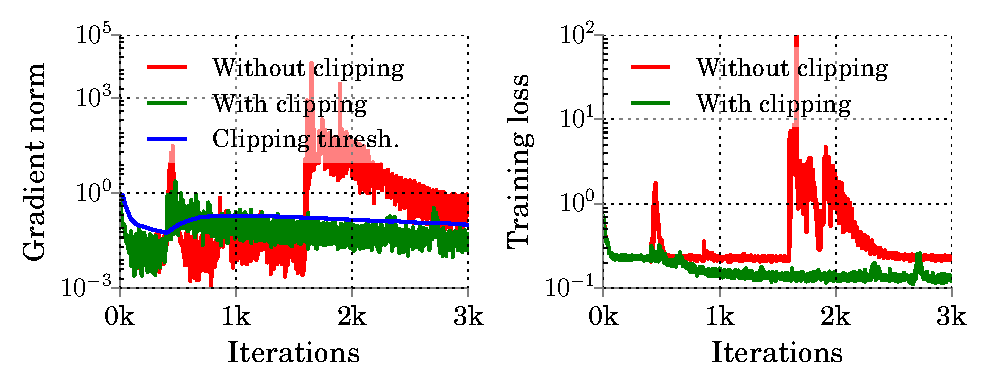
\includegraphics[width=0.95\linewidth]{experiment_results/clipping_example.pdf} 
%% \vspace{-0.75em}
%%\captionof{figure}{A variation of the LSTM architecture in \citep{zhu2016trained} exhibits exploding gradients.
%%The proposed adaptive gradient clipping threshold (blue) stabilizes the training loss.}
%%\label{fig:stability}
%%\end{minipage}
%%\begin{minipage}{0.01\textwidth}
%%	 \ 
%%\end{minipage}
%%\begin{minipage}{0.37\textwidth}
%%\centering
%%%\small
%%\vspace{0.5em}
%%\begin{tabular} {@{\hspace{0.2em}}c | c | c @{\hspace{0.2em}}}
%%\toprule
%%	& Loss & BLEU4 \\
%%\midrule
%%\midrule
%%	Default w/o clip. & \multicolumn{2}{c}{diverge} \\ [0.3em]
%%	Default w/ clip. & 2.86 & 30.75 \\ [0.3em]
%%	YF & \textbf{2.75} & \textbf{31.59} \\
%%\bottomrule
%%\end{tabular}
%%\vspace{2.25em}
%%\captionof{table}{German-English translation validation performance using convolutional seq-to-seq learning.}
%%\label{tab:conv_seq}
%%\end{minipage}
%%%\vspace{-0.75em}
%%\end{table*}
%
%%Section~\ref{sec:oracles} describes the core measurement functions for \tuner tuner. To support its tuning rule, \tuner calculates smoothed, rough approximations of curvature ranges, a distance from a local minimum and gradient variance.
%%Neural network objectives can involve arbitrary non-linearities, and large Lipschitz constants \citep{szegedy2013intriguing}.
%%Furthermore, the process of training them is inherently non-stationary, with the landscape abruptly switching from flat to steep areas. 
%The process of training neural networks is inherently non-stationary, with the landscape abruptly switching from flat to steep areas. 
%In particular, the objective functions of RNNs with hidden units can exhibit occasional but very steep slopes \citep{pascanu2013difficulty,szegedy2013intriguing}.
%%When that happens, the smoothed statistics from our measurement functions might not be representative.
%%So, it is not always safe to assume that the smoothed statistics from our measurement functions so far will accurately represent the objective with abruptly large gradient in the next step.
%To deal with this issue, we use \emph{adaptive gradient clipping} heuristics as a very natural addition to our basic tuner. It is discussed with extensive details in Appendix~\ref{sec:adapt_clip}.  
%In Figure~\ref{fig:stability} in Appendix~\ref{sec:adapt_clip}, we present an example of an LSTM that exhibits the 'exploding gradient' issue. The proposed adaptive clipping can stabilize the training process using \tuner and prevent large catastrophic loss spikes.
%%\begin{table}
%%\centering
%%\begin{tabular} { c | c | c | c}
%%\toprule
%%	& Default w/o clip. & Default w/ clip. & YF \\
%%\midrule
%%\midrule
%%	Validation loss & diverge & 2.86 & 2.75 \\
%%	Validation BLEU4 & diverge & 30.75 & 31.59 \\ 
%%\bottomrule
%%\end{tabular}
%%\caption{German-English translation performance using convolutional sequence to sequence learning.}
%%\label{tab:conv_seq}
%%\end{table}
%
%\begin{wrapfigure}[10]{r}{0.48\linewidth}
%%asdfad
%\hspace{-0.75em}
%\begin{minipage}{\linewidth}
%%%\begin{table}[h]
%%\centering
%\small
%%\hspace{-1em}
%\vspace{-0.75em}
%\begin{tabular} {@{\hspace{0.1em}}c@{\hspace{0.3em}} | @{\hspace{0.35em}}c@{\hspace{0.4em}}c @{\hspace{0.1em}}}
%\toprule
%	& Loss & BLEU4 \\
%\midrule
%\midrule
%	Default w/o clip. & \multicolumn{2}{c}{diverge} \\ [0.3em]
%	Default w/ clip. & 2.86 & 30.75 \\ [0.3em]
%	YF & \textbf{2.75} & \textbf{31.59} \\
%\bottomrule
%\end{tabular}
%%\hspace{-1em}
%\captionof{table}{German-English translation validation metrics using convolutional seq-to-seq model.}
%%\vspace{2.25em}
%\label{tab:conv_seq}
%\end{minipage}
%\end{wrapfigure}
%We validate the proposed adaptive clipping on the convolutional sequence to sequence learning model \citep{gehring2017convolutional} for IWSLT 2014 German-English translation. The default optimizer~\citep{gehring2017convolutional} uses learning rate $0.25$ and Nesterov's momentum $0.99$, diverging to loss overflow due to 'exploding gradient'. It requires, as in~\citet{gehring2017convolutional}, strict manually set gradient norm threshold $0.1$ to stabilize. 
%%We train the model for 120 epochs and report the best validation loss, as well as the best validation BLEU4 score. 
%%We follow the default optimizer setting in~\citep{gehring2017convolutional}, where manually set strict clipping is applied before performing SGD with learning rate $0.25$ and Nesterov's momentum set to $0.99$. 
%%The optimizer diverges when the clipping is removed. 
%In Table~\ref{tab:conv_seq}, we can see YellowFin, with adaptive clipping, outperforms the default optimizer using manually set clipping, with 0.84 higher validation BLEU4 after 120 epochs.
%%Thinking fast and slow approach:
%%- slow layer, the basic tuner we described
%%- fast layer: applies clipping based on the statistics estimated
%%- *and* we don’t let the estimates grow too quickly
%%%%%%%%%%%%%%%%%%%%%%%%%%%%%%%%%%%%%%%%%%%%%%%%%%%%%%%%%%%%%%%%%%%%%%%%%%%%%%%%%


%\begin{table}[t]
%\begin{minipage}{0.62\textwidth}
%\centering
%  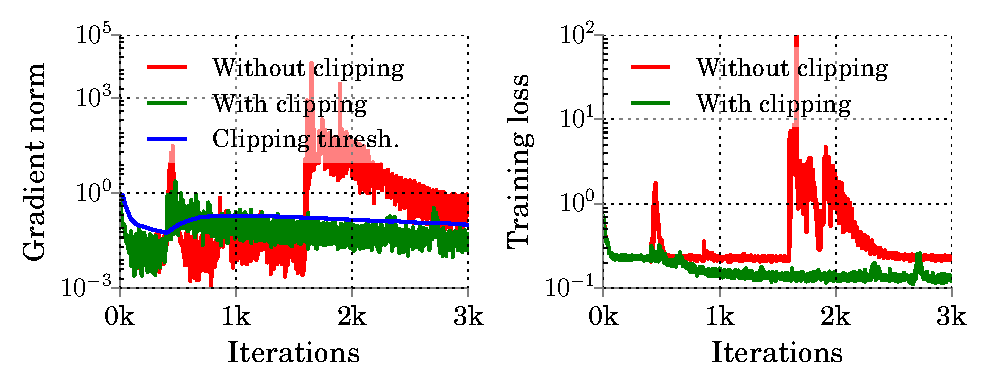
\includegraphics[width=\linewidth]{experiment_results/clipping_example.pdf} 
% \vspace{-1.5em}
%\captionof{figure}{A variation of the LSTM architecture in \citep{zhu2016trained} exhibits exploding gradients.
%The proposed adaptive gradient clipping threshold (blue) stabilizes the training loss.}
%\label{fig:stability}
%\end{minipage}
%\begin{minipage}{0.02\textwidth}
%	 \ 
%\end{minipage}
%\begin{minipage}{0.35\textwidth}
%\centering
%\small
%\vspace{1.5em}
%\begin{tabular} {@{\hspace{0.2em}}c | c | c @{\hspace{0.2em}}}
%\toprule
%	& Loss & BLEU4 \\
%\midrule
%\midrule
%	Default w/o clip. & \multicolumn{2}{c}{diverge} \\ [0.3em]
%	Default w/ clip. & 2.86 & 30.75 \\ [0.3em]
%	YF & \textbf{2.75} & \textbf{31.59} \\
%\bottomrule
%\end{tabular}
%\vspace{1em}
%\caption{German-English translation validation performance using convolutional seq-to-seq learning.}
%\label{tab:conv_seq}
%\end{minipage}
%\end{table}
%
%
%Section~\ref{sec:sync_tuner} describes the core of the \tuner tuner.
%It uses the basic tuning rules extracted from a noisy quadratic model.
%To engineer our implementation on arbitrary objectives, we calculate smoothed, rough approximations of curvature ranges, a distance from a local minimum and gradient variance.
%However, certain neural network objectives can involve arbitrary non-linearities, and large Lipschitz constants \citep{szegedy2013intriguing}.
%Furthermore, the process of training them is inherently non-stationary, with the landscape abruptly switching from flat to steep areas. 
%In particular, the objective functions associated with RNNs   with hidden units can exhibit occasional but very steep slopes \citep{pascanu2013difficulty}.
%So, it is not always safe to assume that the statistics we calculated so far will accurately represent the objective function in the next step.
%
%In Figure~\ref{fig:stability}, we present such an example of an LSTM that exhibits this 'exploding gradient' issue.
%To deal with this issue, we propose a very natural addition to our basic tuner, that performs {\em adaptive gradient clipping}. 
%Gradient clipping has been established in literature as a standard---almost necessary---tool for training such objectives \citep{pascanu2013difficulty,Goodfellow-et-al-2016,gehring2017convolutional}. 
%However, the classic tradeoff between adaptivity and stability applies: 
%setting a clipping threshold that is too low can hurt performance;
%setting it to be high, can compromise stability.
%\tuner, keeps running estimates of extremal gradient magnitude squares, $h_{max}$ and $h_{min}$ in order to estimate a generalized condition number.
%We posit that $\sqrt{h_{max}}$ is an ideal gradient norm threshold for adaptive clipping.
%In order to ensure robustness to extreme gradient spikes, like the ones in Figure~\ref{fig:stability}, we also limit the growth rate of the envelope $h_{max}$ in Algorithm~\ref{alg:curv_func} as follows:
%\begin{equation}
% h_{max} 
% \leftarrow
% \beta \cdot h_{max}
% 	+ (1-\beta) \cdot \textrm{min}\left\{
% 		h_{max,t}, 100 \cdot h_{max}
% 	\right\}
%\end{equation}
%%\begin{table}
%%\centering
%%\begin{tabular} { c | c | c | c}
%%\toprule
%%	& Default w/o clip. & Default w/ clip. & YF \\
%%\midrule
%%\midrule
%%	Validation loss & diverge & 2.86 & 2.75 \\
%%	Validation BLEU4 & diverge & 30.75 & 31.59 \\ 
%%\bottomrule
%%\end{tabular}
%%\caption{German-English translation performance using convolutional sequence to sequence learning.}
%%\label{tab:conv_seq}
%%\end{table}
%
%We demonstrate the performance of YellowFin with adaptive clipping on the IWSLT 2014 German-English translation task using the convolutional sequence to sequence learning model of \citep{gehring2017convolutional}. We train the model for 120 epochs and report the best validation loss, as well as the best validation BLEU4 score. We follow the default optimizer setting in~\citep{gehring2017convolutional}, where manually set strict clipping is applied before performing SGD with learning rate $0.25$ and Nesterov's momentum set to $0.99$. The optimizer diverges when the clipping is removed. In Table~\ref{tab:conv_seq}, we can see YellowFin, with adaptive clipping, can outperform the default optimizer with manually set clipping in both validation loss and BLEU4 score.
%Our proposed adaptive clipping helps stabilize difficult objectives, without sacrificing performance.
%In Appendix~\ref{sec:infl_clip} we demonstrate that on models that do not exhibit instabilities, our clipping does not hurt performance.
%
%%Thinking fast and slow approach:
%%- slow layer, the basic tuner we described
%%- fast layer: applies clipping based on the statistics estimated
%%- *and* we don’t let the estimates grow too quickly
%
